\subsection{Mensagem}

Um software que foi desenvolvido utilizando os conceitos da orientação a
objetos tem sua execução através da comunicação entre os diversos componentes
de software, estes componentes chamados de objetos trocam mensagens com o
objetivo de realizar uma tarefa, isto se faz necessário porque cada objeto  tem
uma responsabilidade para o qual foi projetado na fase de análise.

Assim sendo, uma mensagem é um pedido para que um objeto execute uma ação
através da chamada de um método, sendo que, este pode alterar o estado de
outros objetos a fim de completar a sua tarefa e, quando ele finalmente termina
a sua execução, geralmente notifica quem solicitou a execução do serviço, ou
seja, retorna algum valor para o objeto que solicitou a operação
\cite{c++ComoProgramar}.

Na Figura \ref{fig:mensagem}, é ilustrado o disparo de uma mensagem na linguagem
\acs{PHP}:

\begin{figure}[h!tb]
	\caption{Chamada de um método utilizando a linguagem PHP}
	\label{fig:mensagem}

	\centering
	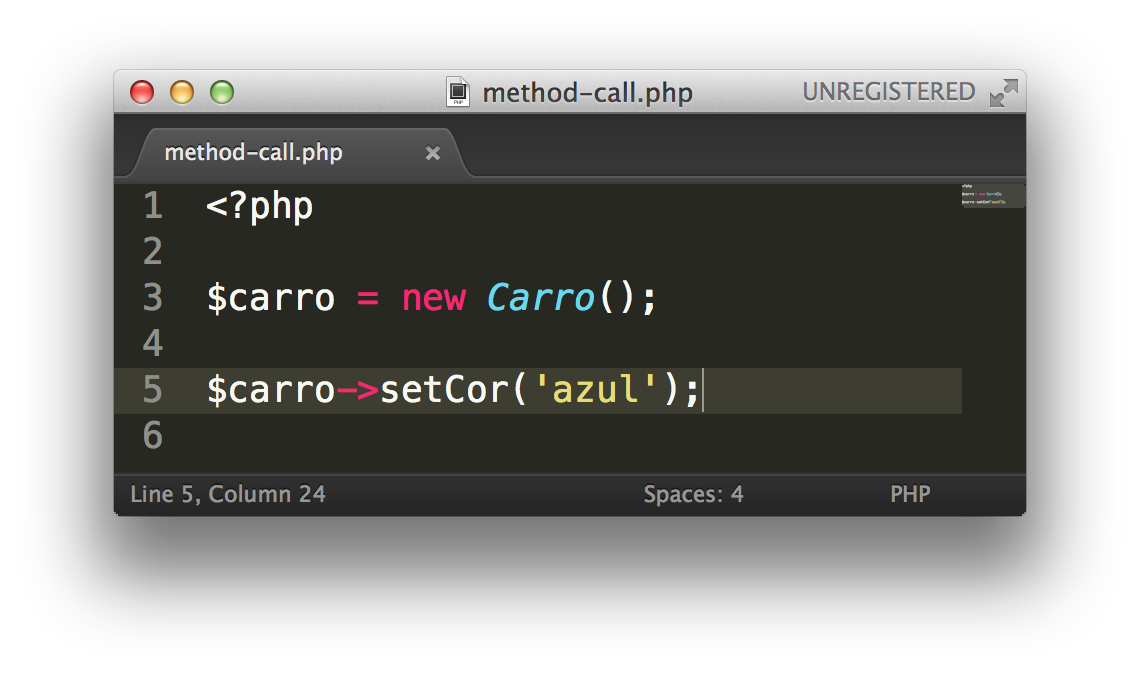
\includegraphics[width=0.6\textwidth]{images/method-call.png}

	\centering
	\footnotesize Fonte: \fonteOAutor
\end{figure}

\FloatBarrier 	% Este comando impede que as imagens
				% flutuem a partir deste ponto no seu documento

A seguir, realiza-se a explicação referente ao código que foi
apresentado na Figura \ref{fig:mensagem}:

\begin{alineas}
    \item linha 1: tem-se o início da execução de um bloco de código
    \acs{PHP};
    \item linha 3: ocorre a criação de um objeto do tipo \textit{Carro};
    \item linha 5: realiza-se a chamada de um método chamado
    \textit{setCor}, sendo que, informa-se um parâmetro para ele, que na
    linguagem \acs{PHP} representa uma \textit{string} (cadeira de caracteres).
    Isto envia uma mensagem para que a classe \textit{Carro} configure
    a propriedade \textit{cor} para receber o valor \textit{azul}.
\end{alineas}

Como foi visto na Figura \ref{fig:mensagem}, o objeto pode invocar um método
público descrito na Classe \textit{Carro} a fim de configurar a cor de um
veículo passando uma mensagem com a cor solicitada.

A seguir, será apresentado o conceito de métodos construtores e como eles podem
colaborar com o desenvolvimento de software inicializando valores de
propriedades.
